\documentclass[a4paper, 12pt]{article}
\usepackage[utf8]{inputenc}
\usepackage[T2A]{fontenc}
\usepackage[ukrainian]{babel}
\usepackage{graphicx}
\usepackage{amsmath}
\usepackage{geometry}
\usepackage{indentfirst}
\geometry{top=2cm, bottom=2cm, left=3cm, right=1.5cm}
\usepackage[colorlinks=true, linkcolor=blue, urlcolor=blue, citecolor=blue]{hyperref}
\begin{document}

\begin{titlepage}
	\begin{center}
		\Large
		\textbf{Київський національний університет імені Тараса Шевченка} \\
		Факультет комп'ютерних наук та кібернетики \\

		\vspace{6cm}

		\textbf{\LARGE ЗВІТ ДО ЛАБОРАТОРНОЇ РОБОТИ №5} \\[0.5cm]
		\textbf{З дисципліни ``Чисельні методи''} \\[0.5cm]
		\textbf{Тема: Природний кубічний інтерполяційний сплайн} \\

		\vfill
		\hspace{7cm} Виконав студент 3-го курсу \\
		\hspace{7cm} групи ТТП-31 \\
		\hspace{7cm} Рісенгін Владислав \\
		\vspace{2cm}

		Київ-2024
	\end{center}
\end{titlepage}

\newpage

\hbadness=99999

\section{Постановка задачі}

Реалізувати природний кубічний інтерполяційний сплайн для функції \( \tan(x) \) на відрізку \([-0.5; 0.5]\). 
Обчислити коефіцієнти сплайну та побудувати графіки:
\begin{itemize}
    \item оригінальної функції,
    \item сплайну,
    \item першої та другої похідних сплайну.
\end{itemize}
Перевірити неперервність сплайну.

\section{Вступ}

Кубічна інтерполяція -- один з найточніших методів наближення функцій, що дозволяє отримати гладку функцію з неперервними першою та другою похідними. Природний кубічний сплайн забезпечує нульові значення другої похідної на краях інтервалу, що часто є природною вимогою.

\section{Деталі реалізації}

Методика побудови природного кубічного сплайну:
\begin{enumerate}
    \item Обчислення кроків \( h_i = x_{i+1} - x_i \).
    \item Побудова матриць:
    \begin{itemize}
        \item Матриці \(C\) для обчислення других похідних \(m\).
        \item Матриці \(H\) для перетворення значень функції у вузлах \(f(x)\) до вигляду правої частини системи.
    \end{itemize}
    \item Розв’язання системи \(C \cdot m = b\), де \(m\) -- вектор других похідних.
    \item Визначення коефіцієнтів \(A_i, B_i\) для кожного сегмента.
    \item Обчислення значень сплайну за формулою:
    \[
    S_i(x) = \frac{(x_i - x)^3}{6h_i}m_{i-1} + \frac{(x - x_{i-1})^3}{6h_i}m_i + A_i \frac{x - x_{i-1}}{h_i} + B_i \frac{x_i - x}{h_i}.
    \]
    \item Побудова графіків для аналізу результатів.
\end{enumerate}

\clearpage
\section{Теоретичний опис методів}

Основні етапи розв’язання задачі:
\begin{itemize}
    \item \textbf{Матриця \(C\):} тридіагональна матриця для знаходження других похідних \(M\), елементи якої визначаються кроками \(h_i\):
    \[
    C_{i, i-1} = \frac{h_{i-1}}{6}, \quad C_{i, i} = \frac{h_{i-1} + h_i}{3}, \quad C_{i, i+1} = \frac{h_i}{6}.
    \]
    \item \textbf{Матриця \(H\):} використовується для побудови правої частини:
    \[
    H_{i, i-1} = \frac{1}{h_{i-1}}, \quad H_{i, i} = -\left(\frac{1}{h_{i-1}} + \frac{1}{h_i}\right), \quad H_{i, i+1} = \frac{1}{h_i}.
    \]
    \item \textbf{Система рівнянь:}
    \[
    b = H \cdot f(x).
    \]
    Далі розв’язується система \(C \cdot m = b\).
\end{itemize}

\newpage
\section{Результати роботи програми}

На основі реалізації програми було отримано наступні результати:

\subsection{Вузли інтерполяції}

Вузли \(x\) і відповідні значення функції \(y = \tan(x)\): \\

\(x =  [ -0.5 , -0.4286 , -0.3571 , -0.2857 , -0.2143 , -0.1429 , -0.0714 , \)

\( 0 , 0.0714 , 0.1429 , 0.2143 , 0.2857 , 0.3571 , 0.4286 , 0.5 ] \)


\(y = [-0.5463 , -0.4569 , -0.3731 , -0.2938 , -0.2176 , -0.1438 , -0.0716 , 0 \)

\(0.0716 , 0.1438 , 0.2176 , 0.2938 , 0.3731 , 0.4569 , 0.5463 ] \)

\(h = [0.0714 , 0.0714 , 0.0714 , 0.0714 , 0.0714 , 0.0714 , 0.0714 \)

\(0.0714 , 0.0714 , 0.0714 , 0.0714 , 0.0714 , 0.0714 ] \)

\subsection{Матриця \(C\)}
Тридіагональна матриця коефіцієнтів \(C\):

\begin{figure}[h!]
    \centering
    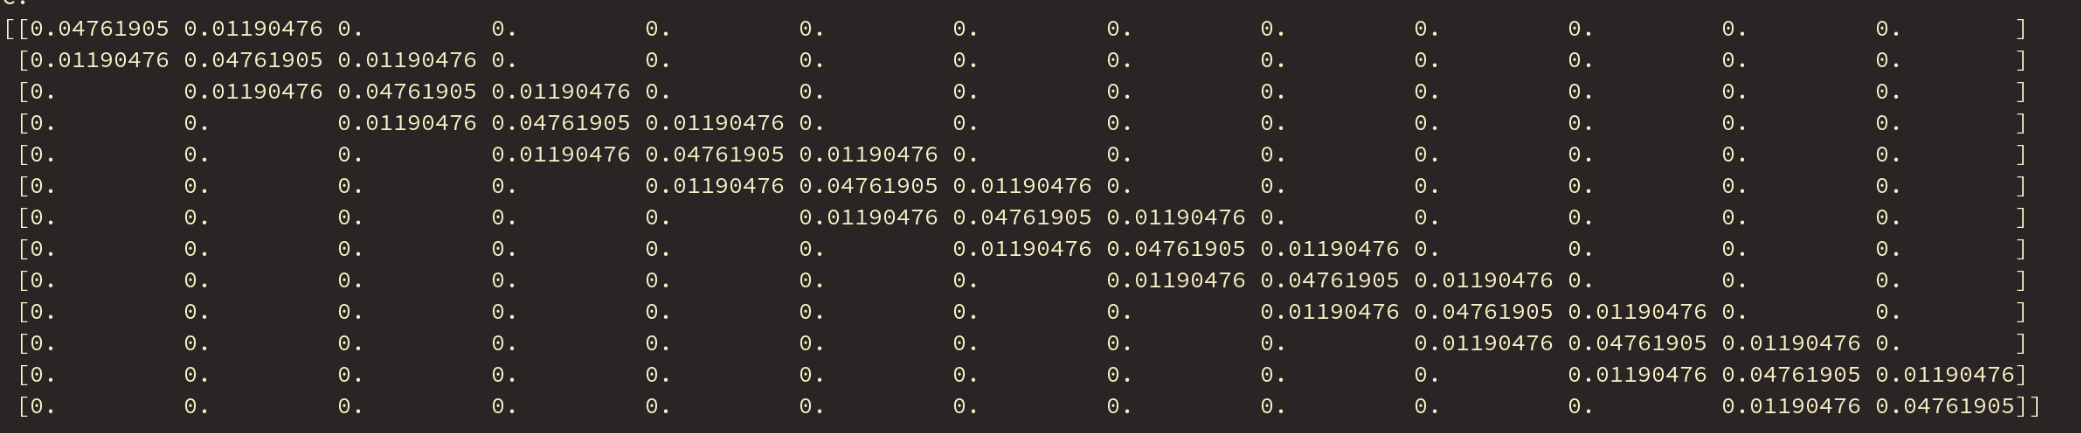
\includegraphics[width=0.9\textwidth]{C.png}
    \label{fig:C}
\end{figure}

\subsection{Матриця \(H\)}
Тридіагональна матриця коефіцієнтів \(H\):

\begin{figure}[h!]
    \centering
    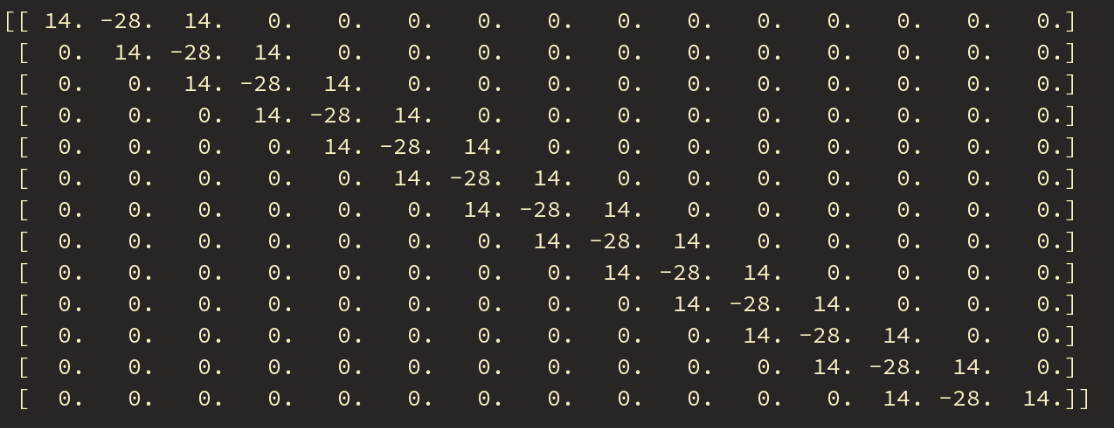
\includegraphics[width=0.9\textwidth]{H.png}
    \label{fig:H}
\end{figure}

\newpage
\subsection{Інші вектори}

\( b = [ -0.0792 , -0.0610 , -0.0458 , -0.0327 , -0.0210 , -0.0103  \) 

\( 0 , 0.0103 , 0.0210 , 0.0327 , 0.0458 , 0.0610 , 0.0792 ] \)

\( m = [ 0 , -1.4779 , -0.7454 , -0.6629 , -0.4469 , -0.2945 , -0.1429 \) 

\( 0 , 0.1429 , 0.2945 , 0.4469 , 0.6629 , 0.7454 , 1.4779 , 0 ] \)

\( A = [ -0.5463 , -0.4556 , -0.3725 , -0.2932 , -0.2172 , -0.1436 , -0\) 

\( 14 , 0 , 0.0714 , 0.1436 , 0.2172 , 0.2932 , 0.3725 , 0.4556 ] \)

\( B = [ -0.4556 , -0.3725 , -0.2932 , -0.2172 , -0.1436 , -0.0714 , 0 \) 

\( 0.0714 , 0.1436 , 0.2172 , 0.2932 , 0.3725 , 0.4556 , 0.5463 ] \)

\subsection{Сплайн}
\(S(x) = \)
\[
\begin{cases}
-3.448436 * x^3 + 0.000000 * x^2 + 1.269325 * x + -0.546302, & x \in [-0.500000, -0.428571) \\
1.709264 * x^3 + -0.738950 * x^2 + 1.216543 * x + -0.455636, & x \in [-0.428571, -0.357143) \\
0.192374 * x^3 + -0.372680 * x^2 + 1.137141 * x + -0.372511, & x \in [-0.357143, -0.285714) \\
0.503941 * x^3 + -0.331457 * x^2 + 1.086846 * x + -0.293188, & x \in [-0.285714, -0.214286) \\
0.355599 * x^3 + -0.223469 * x^2 + 1.047208 * x + -0.217247, & x \in [-0.214286, -0.142857) \\
0.353925 * x^3 + -0.147269 * x^2 + 1.020727 * x + -0.143587, & x \in [-0.142857, -0.071429) \\
0.333332 * x^3 + -0.071428 * x^2 + 1.005106 * x + -0.071429, & x \in [-0.071429, 0.000000) \\
0.333332 * x^3 + -0.000000 * x^2 + 1.000003 * x + 0.000000, & x \in [0.000000, 0.071429) \\
0.353925 * x^3 + 0.071428 * x^2 + 1.005106 * x + 0.071429, & x \in [0.071429, 0.142857) \\
0.355599 * x^3 + 0.147269 * x^2 + 1.020727 * x + 0.143587, & x \in [0.142857, 0.214286) \\
0.503941 * x^3 + 0.223469 * x^2 + 1.047208 * x + 0.217247, & x \in [0.214286, 0.285714) \\
0.192374 * x^3 + 0.331457 * x^2 + 1.086846 * x + 0.293188, & x \in [0.285714, 0.357143) \\
1.709264 * x^3 + 0.372680 * x^2 + 1.137141 * x + 0.372511, & x \in [0.357143, 0.428571) \\
-3.448436 * x^3 + 0.738950 * x^2 + 1.216543 * x + 0.455636, & x \in [0.428571, 0.500000] \\
\end{cases}
\]

\newpage
\subsection{Графіки}
Було побудовано наступні графіки:

\begin{figure}[h!]
    \centering
    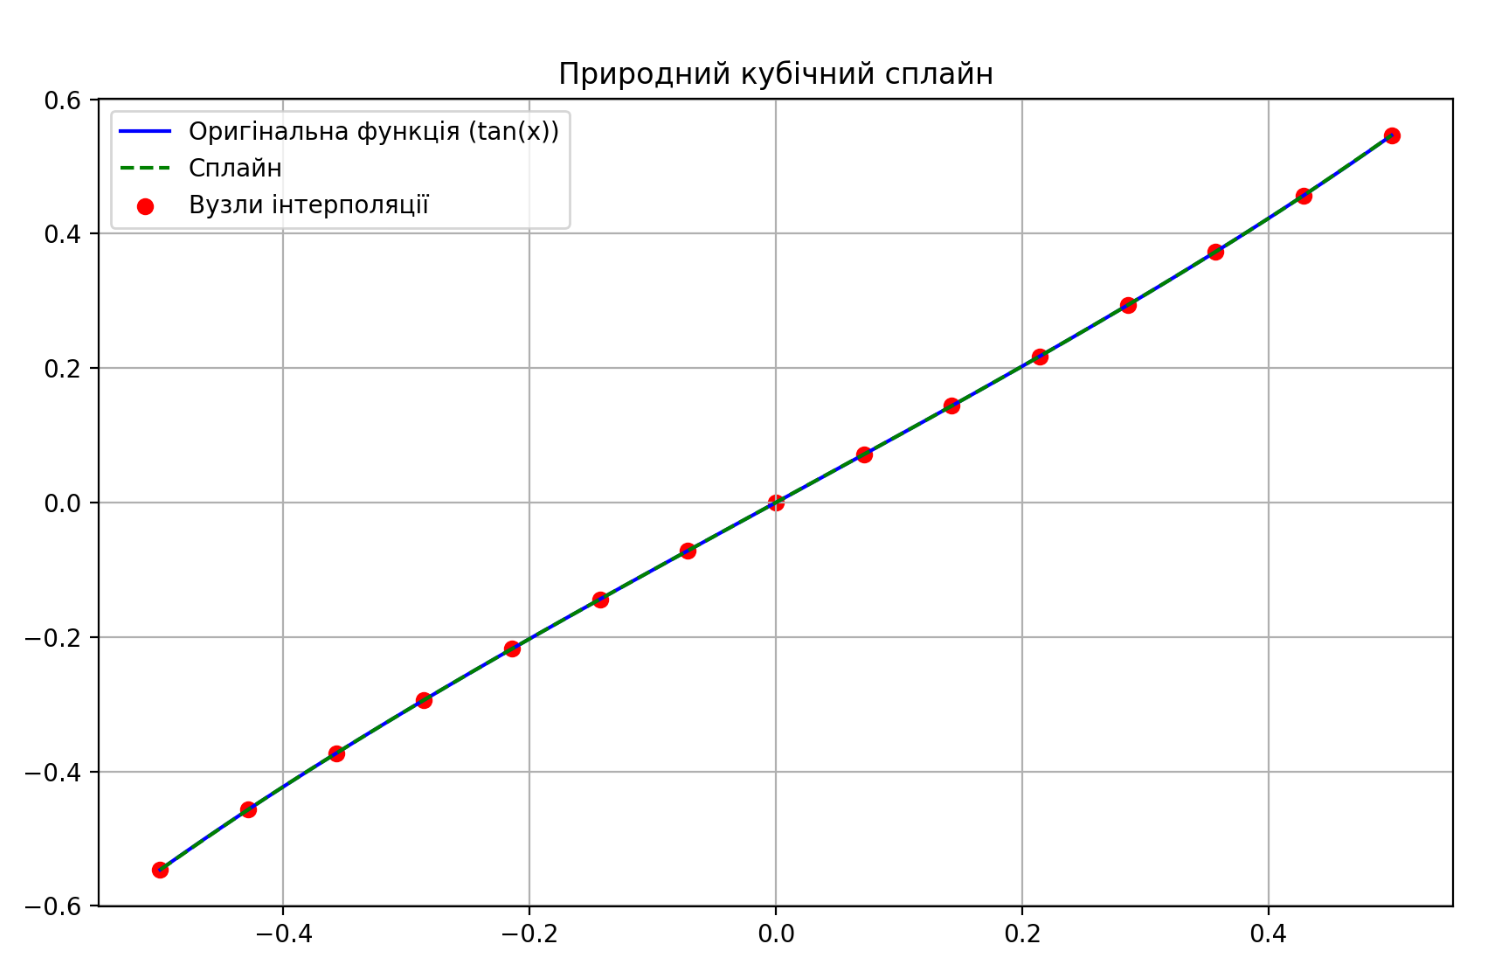
\includegraphics[width=0.9\textwidth]{spline_plot.png}
    \caption{Графіки оригінальної функції \( \tan(x) \) та інтерполяційного сплайну}
    \label{fig:spline}
\end{figure}

\begin{figure}[h!]
    \centering
    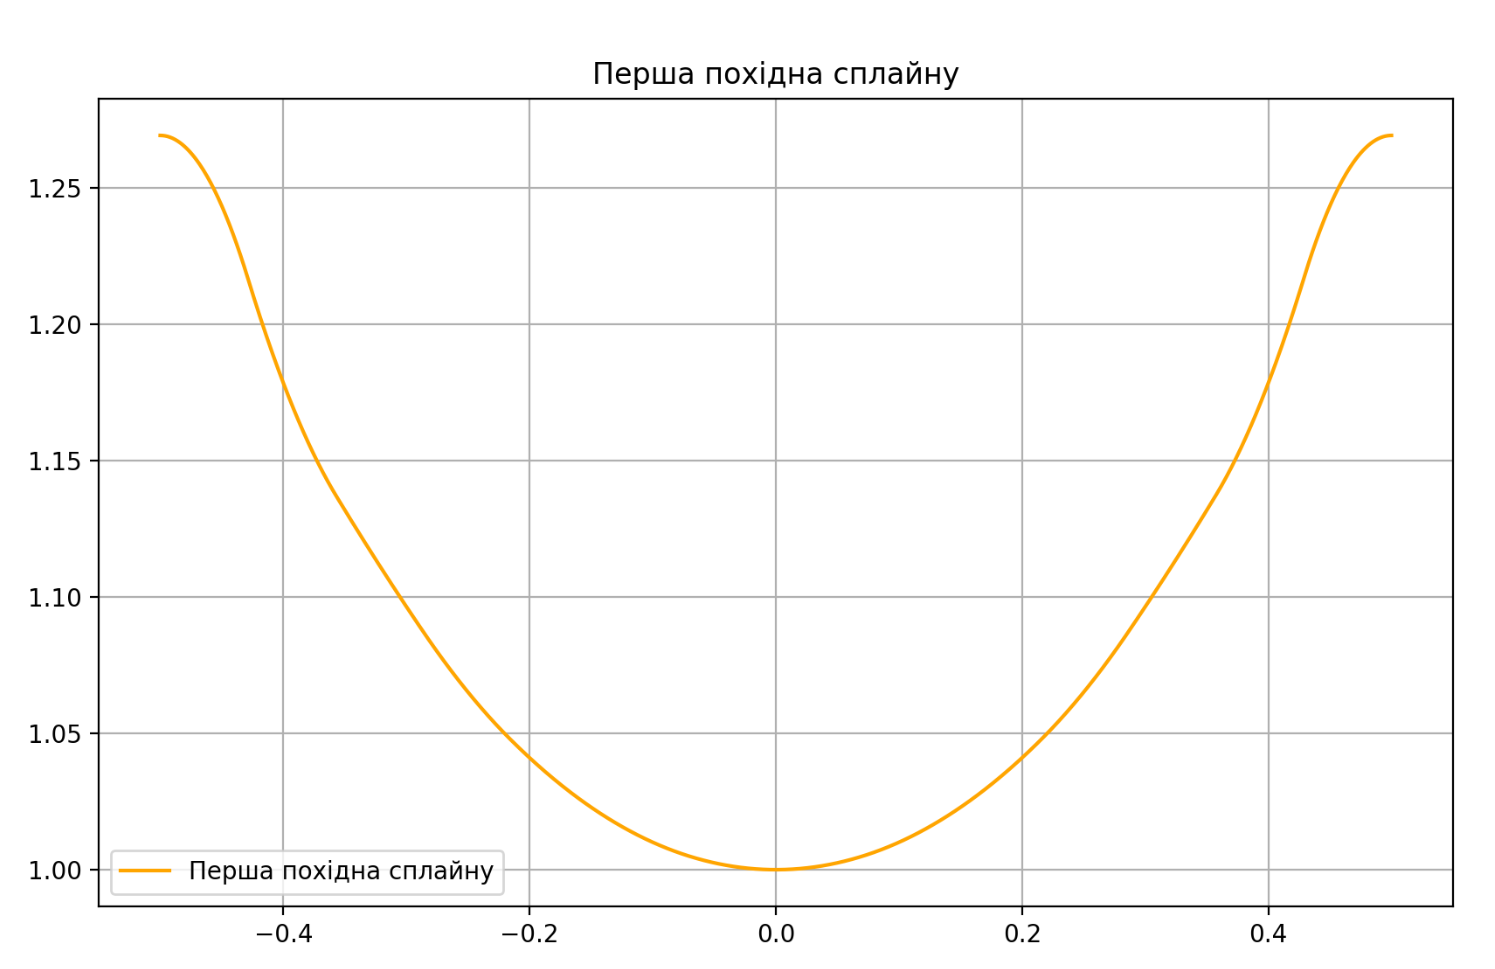
\includegraphics[width=0.9\textwidth]{first_der.png}
    \caption{Графік першої похідної інтерполяційного сплайну}
    \label{fig:first_der}
\end{figure}

\begin{figure}[h!]
    \centering
    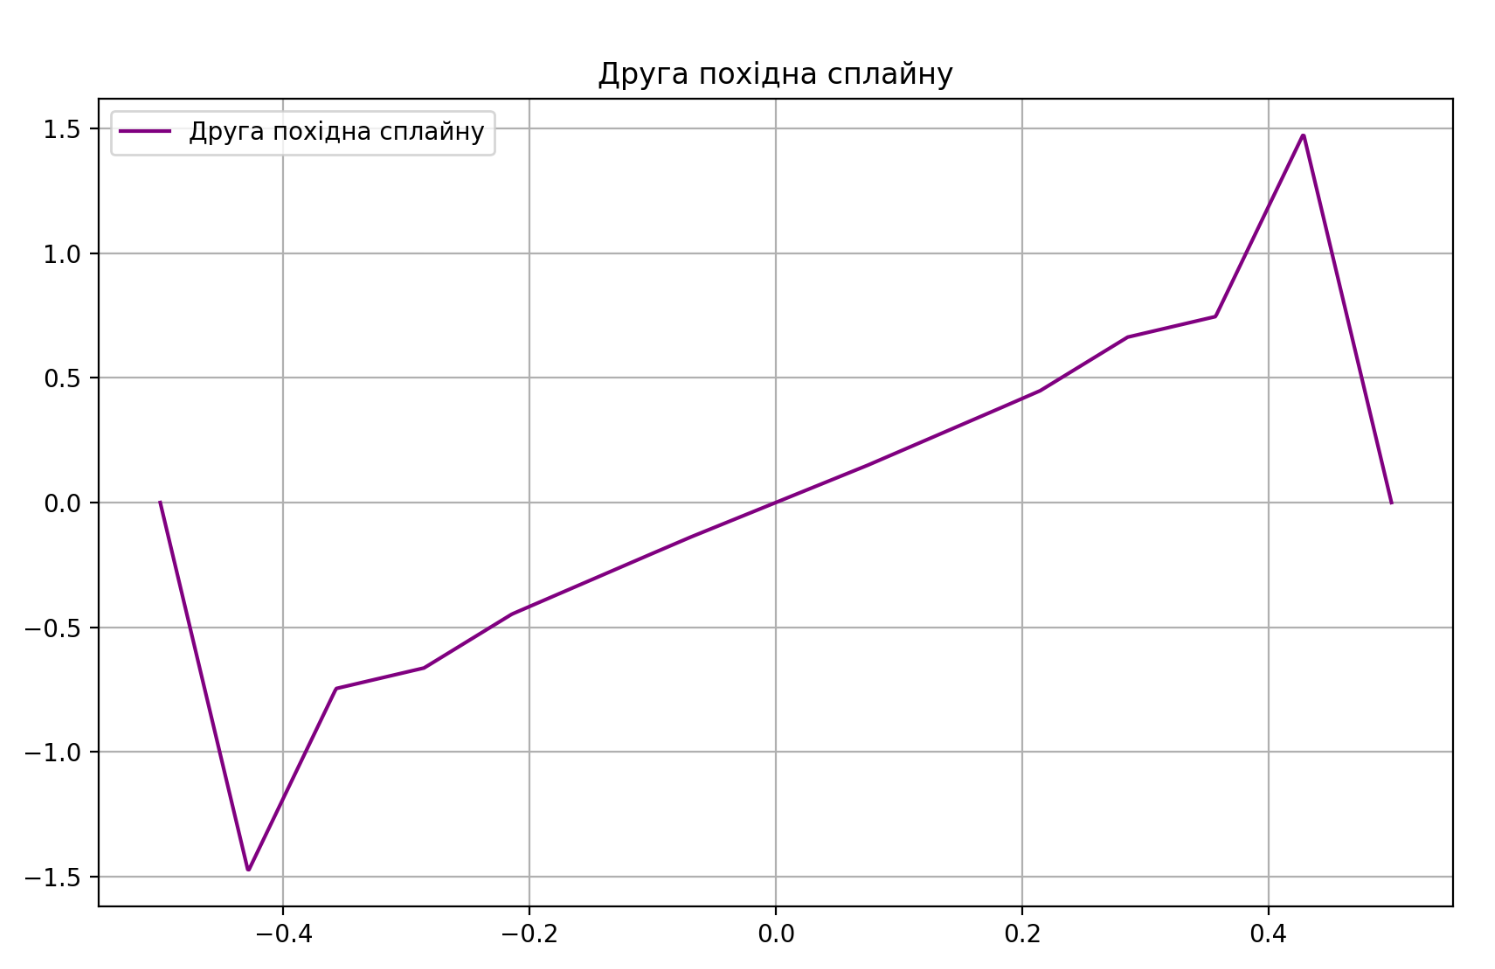
\includegraphics[width=0.9\textwidth]{second_der.png}
    \caption{Графік другої похідної інтерполяційного сплайну}
    \label{fig:second_der}
\end{figure}



\clearpage
\newpage
\section{Висновок}

У ході виконання роботи був побудований природний кубічний сплайн для функції tan(x), який задовольняє всім основним умовам сплайну: умовам неперервності, гладкості першої похідної, а також природним граничним умовам. Сплайн дозволив виконати інтерполяцію з високою точністю, забезпечуючи значно кращі результати, ніж використання звичайного полінома Ньютона. 

Поліноми високого ступеня, такі як поліном Ньютона, часто страждають від ефекту Рунге, що призводить до великих похибок на краях інтервалу. Натомість, кубічний сплайн, завдяки своїй конструкції, ділить інтервал на сегменти, кожен з яких моделюється поліномом третього ступеня. Такий підхід дає змогу уникнути значних коливань та суттєво знижує похибку.

Загалом, метод побудови кубічних сплайнів є надзвичайно ефективним і потужним інструментом для задач інтерполяції. Він дозволяє точно апроксимувати складні гладкі функції та знаходить застосування в різних галузях, зокрема в чисельному аналізі, обробці сигналів та комп’ютерній графіці. Результати виконаної роботи підтвердили, що сплайни є надійним та універсальним методом, який можна рекомендувати для використання у задачах, де потрібна точна інтерполяція.

\end{document}
